In the sequel we assume that $L_1 = L_2 = \dots = L_t \triangleq L$  in the surveillance game structure, i.e, all $n$ sensors and the target operate in the same state space. For the remainder of the paper, let $G=(\states,s^\init,\trans,\vis_1,\ldots,\vis_n)$ be a multi-agent surveillance game structure  defined over  $L$.

\begin{figure}
A  \emph{state-space partition} of size $n$ of the set $L$ of locations in a game structure $G$ is tuple $\widetilde L =  (\widetilde L_1,\ldots,\widetilde L_n)$ of subsets of $L$ such that  $\bigcup_i^n L_i = L $, and $\widetilde L_i \cap \widetilde L_j  = \emptyset$ for $i \neq j$. 

\subfloat[Surveillance game partitioned into two subgames \label{part-grid}]{
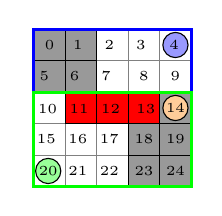
\begin{tikzpicture}[scale=0.8]
\draw[step=0.5cm,color=gray] (-1.5,-1.5) grid (1,1);
\filldraw[fill=red,draw=black] (0,0) rectangle (-0.5,-0.5);
\filldraw[fill=red,draw=black] (-0.5,0) rectangle (-1,-0.5);
\filldraw[fill=red,draw=black] (0,0) rectangle (0.5,-0.5);
\filldraw[fill=gray!80!white,draw=black] (-0.5,0.5) rectangle (-1,1);
\filldraw[fill=gray!80!white,draw=black] (-0.5,0) rectangle (-1,0.5);
\filldraw[fill=gray!80!white,draw=black] (-1,0.5) rectangle (-1.5,1);
\filldraw[fill=gray!80!white,draw=black] (-1,0) rectangle (-1.5,0.5);
\filldraw[fill=gray!80!white,draw=black] (0.5,-0.5) rectangle (1,-1);
\filldraw[fill=gray!80!white,draw=black] (0,-0.5) rectangle (0.5,-1);
\filldraw[fill=gray!80!white,draw=black] (0,-1) rectangle (0.5,-1.5);
\filldraw[fill=gray!80!white,draw=black] (0.5,-1) rectangle (1,-1.5);
\filldraw[fill=gray!80!white,draw=black] (0.5,-0.5) rectangle (1,0);

\filldraw[fill=blue!40!white,draw=black] (+0.75,+0.75) circle (0.2cm);
\filldraw[fill=orange!40!white,draw=black] (0.75,-0.25) circle (0.2cm);
\filldraw[fill=green!40!white,draw=black]  (-1.27,-1.25) circle (0.2cm);
\filldraw[fill=none,draw=blue,line width=0.4mm] (-1.5,0) rectangle (1,1);
\filldraw[fill=none,draw=green,line width=0.4mm] (-1.5,-1.5) rectangle (1,0);
\node at (-1.25,+0.75) {\tiny{0}};
\node at (-0.80,+0.75) {\tiny{1}};
\node at (-0.30,+0.75) {\tiny{2}};
\node at (0.20,+0.75) {\tiny{3}};
\node at (0.73,+0.75) {\tiny{4}};
\node at (-1.33,+0.25) {\tiny{5}};
\node at (-0.85,+0.25) {\tiny{6}};
\node at (-0.35,+0.25) {\tiny{7}};
\node at (0.25,+0.25) {\tiny{8}};
\node at (0.75,+0.25) {\tiny{9}};
\node at (-1.28,-0.27) {\tiny{10}};
\node at (-0.78,-0.27) {\tiny{11}};
\node at (-0.28,-0.27) {\tiny{12}};
\node at (0.28,-0.27) {\tiny{13}};
\node at (0.75,-0.25) {\tiny{14}};
\node at (-1.3,-0.75) {\tiny{15}};
\node at (-0.8,-0.75) {\tiny{16}};
\node at (-0.3,-0.75) {\tiny{17}};
\node at (0.25,-0.75) {\tiny{18}};
\node at (0.75,-0.75) {\tiny{19}};
\node at (-1.27,-1.25) {\tiny{20}};
\node at (-0.8,-1.25) {\tiny{21}};
\node at (-0.3,-1.25) {\tiny{22}};
\node at (0.25,-1.25) {\tiny{23}};
\node at (0.75,-1.25) {\tiny{24}};

\end{tikzpicture}
\hspace{.3cm}}
%\hfill
\subfloat[Possible transitions from current state in each subgame \label{part-grid-trans}]{

\begin{minipage}{5.0cm}
\vspace{-2.8cm}
%{\fontsize{8}{10}\selectfont $\Vis((20,4),18) = \false,\vis(4,17) = \false,$ $\vis(4,19) = \true, \vis(4,23) = \false$}

%\smallskip

%\small \[\tilde{L} =\begin{cases}
%\widetilde{L}_1 = \{0,1,2,3,4,5,6,7,8,9\} \\
%\widetilde{L}_2 = \{10,11,12,13,14,\ldots,24\}
%
%\end{cases}\]


\begin{tikzpicture}[node distance=.9 cm,auto,>=latex',line join=bevel,transform shape,scale=.75]
\node at (0,0) (s0) {$G^1: (20,14)$};
\node  [below left of=s0,yshift=-.5cm,xshift=-0.5cm] (s2) {$(21,k_1)$};
\node  [below right of=s0,yshift=-.5cm,xshift=0.5cm] (s3) {$(15,k_1)$};
\node  [left of=s2,xshift=-0.75cm] (s1) {$(21,\{19\})$};
\node  [right of=s3,xshift=0.75cm] (s4) {$(15,\{19\})$};
\draw [->] (s0) edge (s1.north);
\draw [->] (s0) edge (s2.north);
\draw [->] (s0) edge (s3.north);
\draw [->] (s0) edge (s4.north);
\end{tikzpicture}



\begin{tikzpicture}[node distance=.9 cm,auto,>=latex',line join=bevel,transform shape,scale=.75]
\node at (0,0) (s0) {$G^2: (4,k_1)$};
\node  [below of=s0,yshift=-.5cm] (s1) {$(3,9)$};
\node  [right of=s1,xshift=0.5cm] (s2) {$(9,k_2)$};
\node  [left of=s1,xshift=-0.5cm] (s3) {$(3,k_2)$};
\draw [->] (s0) edge (s1.north);
\draw [->] (s0) edge (s2.north);
\draw [->] (s0) edge (s3.north);
\end{tikzpicture}



\end{minipage}
}


\caption{Partitioning of the state space of a surveillance game into two subgames comprising of states $\widetilde{L}_1$ - green and $\widetilde{L}_2 - blue$. }
\label{fig:simple-dist-game}
\end{figure}

\subsection{Surveillance subgames}
We now describe how, given a state-space partition $\widetilde L =  (\widetilde L_1,\ldots,\widetilde L_n)$, to construct a tuple of single-agent surveillance game structures $\widetilde G = (G_1,\ldots,G_n)$ that contains one  \emph{surveillance subgame} $G^i$ for each mobile sensor  $i$. Each subgame, $G^i$ is defined over the subset of locations $\widetilde{L}_i$. Since the target and sensor operate on the same state space we will have $\widetilde{L}^i_s = \widetilde{L}^i_t = \widetilde{L}_i$. Additionally, to each $\widetilde{L}^i_t$ we add an \emph{auxiliary location} $k_i$ that encapsulates all possible locations of the target that are outside of this subgame's region, i.e., all locations in $L \setminus \widetilde{L}_i$.  We then model transitions leaving or entering $\widetilde{L}^i_t$ as transitions to or from location $k_i$ respectively.

More formally, given the subset  $\widetilde{L}_i \subseteq L$ we define the \emph{subgame} of $G$ corresponding to sensor $i$ as the tuple $G^i = (\widetilde{S}_i,\widetilde{s}_i^{init},\widetilde{T}_i,\widetilde{\vis}_i)$  where
\begin{itemize}
\item $\widetilde{S}_i= \widetilde{L}_i \times (\widetilde{L}^i_t \cup k_i)$ is the set of states.
\item The set $\widetilde{T}_i$ consists of two types of transitions: the transitions in $T{\downarrow } i$ that originate and end in locations that are part of the subgame's region are preserved as they are, while the transitions of the target exiting or entering $\widetilde{L}^i_t$ are replaced by transitions to and from location $k_i$ respectively, since $k_i$ represents all target locations outside of  $\widetilde{L}^i_t$. 
Formally, for every pair of states $(\widetilde{l}_i,\widetilde{l}_t) \in \widetilde{S}_i$ and $(\widetilde{l}_i',\widetilde{l}_t') \in \widetilde{S}_i$ we have that $((\widetilde{l}_i,\widetilde l_t),(\widetilde{l}_i',\widetilde l_t')) \in \widetilde T_i$ if and only if there exists a transition
 $((\widetilde{l}_i,l_t),(\widetilde{l}_i',l_t')) \in T{\downarrow}i$ for which the following conditions are satisfied:
 \begin{itemize}
 \item if $\widetilde l_t \in \widetilde L_t ^i$ and $\widetilde l_t' \in \widetilde L_t ^i$, then 
 $\widetilde l_t = l_t$ and $\widetilde l_t'= l_t'$, that is, we have a \emph{transition internal for the region $\widetilde L_t^i$};
 \item if $\widetilde l_t \in \widetilde L_t ^i$ and $\widetilde l_t' =  k_i$, then 
 $l_t \in \widetilde L_t^i$ and $l_t' \not\in \widetilde L_t^i$, that is, we have a \emph{transition exiting the region $\widetilde L_t^i$}; 
 \item if $\widetilde l_t= k_i$ and $\widetilde l_t' \in  \widetilde L_t ^i$, then 
 $l_t \not \in \widetilde L_t^i$ and $l_t' \in \widetilde L_t^i$, that is, we have a \emph{transition entering the region $\widetilde L_t^i$}; 
 \item if $\widetilde l_t= k_i$ and $\widetilde l_t' =  k_i$, then 
 $l_t \not \in \widetilde L_t^i$ and $l_t' \not\in \widetilde L_t^i$, that is, we have a \emph{transition completely outside $\widetilde L_t^i$}.
\end{itemize}  

  \item The visibility function $\widetilde{\vis}_i$ in the subgame $G^i$ agrees with the visibiity function $\vis_i$ of sensor $i$ in the original game when the target's location is in the subgame's region. Target locations outside of the region $\widetilde L_t^i$  (summarized by location $k_i$) are invisible to the sensor in the subgame. Formally, 
 \[\widetilde{\vis}_i(\widetilde{l}_i,l_t) = \begin{cases}
\vis_i(\widetilde{l}_i,l_t) & l_t \in \widetilde{L}_t^i, \\
\false & l_t  = k_i.
\end{cases}
\]
\end{itemize}
\begin{example}
In Figure \ref{part-grid}, we have two subgames: $G^1$ for the green sensor and $G^2$ for the blue one. The states in the subgames are $s_1 = (20,14)$, and $s_2 = (4,k_2)$ . Recall that $k_i$ is an indicator state to represent that the target is not subgame $i$. The possible transitions shown in \ref{part-grid-trans} show that the target has the ability to either leave $G^1$ and enter $G^2$. 
%Finally recall that in example \ref{ex:simple-surveillance-game}, we had state $Vis((20,4),14) = \true$. This is no longer the case as although we have $\vis_1(4,14) = \true$ in the global game (i.e, it is visible to sensor 1 and hence also visible to the entire sensor network), state 14 does not lie in $\widetilde{L}_1$ which means it is not visible in the subgame for sensor 1.
\qed
\end{example}

Note that in this construction, sensor $i$ is not able to leave the region of locations $\widetilde{L}_i$. Furthermore, all the information about the target's behaviour outside of  the subgame's region is completely hidden from the mobile sensor controller, since all locations outside of  $\widetilde{L}_t^i$ are represented by the single location $k_i$.
Finally we remark that the previously defined notions of $\succs_t(\widetilde{l}_i,\widetilde{l}^i_{t})$, $\succs_t(\widetilde{l}_i,\widetilde{L}^i_{t})$, and $\succs(\widetilde{l}_i,\widetilde{l}^{t},\widetilde{l}_{t}')$ for the global game structure $G$ follow analogously in this construction for $\widetilde{T}$ which we denote as $\widetilde{\succs}$.

\subsection{Belief subgame}
\Rayna{I think we should define in the previous section single-agent surveillance game structures as a special case of multi-agent surveillance game structures. Then, since a surveillance subgame is essentially a single-agent surveillance game, and since there is nothing specific in the definition below, we can remove this subsection and  move the last remark to the next subsection.}
Given a surveillance subgame $G^{i} = (\widetilde{S}_i,\widetilde{s}_i^{init},\widetilde{T}_i,\widetilde{\vis}_i)$, we can construct a belief subgame $G^{i}_\belief = (\widetilde{\states}_{i_\belief},\widetilde{s}^\init_{i_\belief},\widetilde{\trans}_{i_\belief})$ 

\begin{itemize}
\item $\states_{i_\belief} = \widetilde{L}_i \times \mathcal{P}(\widetilde{L}^i_t \cup k_i)$ is the set of states,
\item $\widetilde{\trans}_{i_\belief} \subseteq \widetilde{\states}_{i_\belief} \times \widetilde{\states}_{i_\belief}$ is the transition relation where $((\widetilde{l}_i, B_t),(\widetilde{l}_i', B_t')) \in \widetilde{\trans}_{i_\belief}$ iff $\widetilde{l}_i' \in  \widetilde{\succs}(\widetilde{l}_i,l_t,l_t')$ for some $l_t \in B_t$ and $l_t' \in B_t'$ and one of these holds:
\begin{itemize}
\item[(1)] $B_t' = \{l_t'\}$, $l_t' \in \widetilde{\post}(\widetilde{l}_i,B_t)$, $\widetilde{\vis}_i(l,l_t') = \true$;
\item[(2)] $B_t' = \{l_t' \in \widetilde{\post}(\widetilde{l}_i,B_t)  \mid  \widetilde{\vis}_i(l,l_t') = \false \}$.
%\item[(1)] $B_t' = \{l_t'\}$ for some $l_t'$ such that $\vis(l_a,l_t') = \true$ and
%there exists $l_t \in B_t$ with $((l_a,l_t),(l_a',l_t')) \in \trans$;
%\item[(2)] $\begin{array}{lll}
%B_t' = \{l_t' & \mid & \vis(l_a,l_t') = \false \text{ and } \\
%&& \exists l_t \in B_t.\ ((l_a,l_t),(l_a',l_t')) \in \trans\}. 
%\end{array}
%$
\end{itemize}
\end{itemize}

 For brevity, we omit the definitions of $\widetilde{\succs}_t$, $\widetilde{\succs}$, runs and strategies for the belief subgames as the definitions follow trivially from those for the belief games but in the subspace of transitions and states as defined above.

The outcome of given strategies $f_{i}$ and $f_{t_i}$ for sensor $i$ and the target in the subgame, $\outcome(G^{i}_{\belief},f_s,f_t)$, is a run $s_0,s_1,\ldots$ of $G^{i}_\belief$ such that for every $k \geq 0$, we have $s_{k+1} = f_i(s_0,\ldots,s_k,B^k_{t_i})$, where $B^k_{t_i} = f_{t_i}(s_0,\ldots,s_k)$.

\paragraph*{Remark}$B^k_{t_i}$ is the belief that sensor $i$ holds on the position of the target. Since the subgame for each sensor will be executing concurrently, the global belief on the location of the target will be a combination of the knowledge of the individual sensors. This is discussed in more detail in the sequel.

\subsection{Composition of subgames}
Given $n$ belief subgames $(G^{1}_{\tilde{S}_\belief},\ldots,G^{n}_{\tilde{S}_\belief})$ over state partition $\widetilde{L}$, we define a \emph{run} in the composed belief game $G_\belief$ as an infinite sequence $s_0,s_1,\ldots$ of states where $s_k = (\tilde{s}_{1_k} \ldots \tilde{s}_{n_k})$ is the combined state of all the subgames at timestep $k$, and  $(\tilde{s}_{i_k},\tilde{s}_{{i+1}_k}) \in \tilde{T}_{i_\belief}$ for all $k$. 

Given a strategy for each sensor $f_{s_i}$ in the corresponding subgames, we compose the subgame strategies into a global strategy in the same way. 


\subsection{Global belief vs local belief}

Given $n$ belief subgames, at timestep $k$, sensor $i$ holds belief $B^k_{t_i}$. This is the \emph{local} belief as it is held by a single sensor and is not shared with the others. We first present the following fact: \todo{\textbf{not sure if this is a theorem, but not sure what else to call it.}}
\begin{theorem} 
At timestep $k$, if there exists $i\in \{1\dots n\}$ such that $B^k_{t_i} = \{l_t\}$ for $l_t \in \widetilde{L}_i^t$, then for all $j \neq i$, we have $k_j \in B^k_{t_j}$.
\end{theorem}
\begin{proof}
By construction of the subgames \textbf{more to come}
\end{proof}
\begin{corollary}\label{corr:uniqi}
There can exist at most one $i\in \{1\dots n\}$ such that $B|^k_{t_i}| = 1$ and $k_j \in B^k_{t_j} \notin B|^k_{t_i}|$.
\end{corollary}
Intuitively, this states that if the target is in vision of sensor $i$, all the other sensors must have $k_j$ in their belief sets. Recall that $k_j$ indicates that the target is not in the state space of the subgame corresponding to sensor $j$. The corollary states that if the target is in vision of sensor $i$, then no other sensor can claim to see the same target. 
The global belief is defined as:
\[B^k_t \triangleq 
\bigcap_{i}^n B^k_{t_i}
\]

 




\subsection{Distributed surveillance synthesis problem}
\paragraph*{\textbf{Problem statement: }}Given a global surveillance game $(G,\varphi)$ with $n$ sensors and a state partition $\widetilde{L}$, compute a distributed strategy for the sensor in each subgame $G^i_\belief$ such that the composition of the $n$ subgame strategies guarantees that the global surveillance objective $\varphi$ is satisfied. Formally, compute the strategy $f_i$ for the sensor in each belief subgame such that $f_s = f_{s_1} \bigoplus f_{s_2} \dots \bigoplus f_{s_n}$ must be winning for the global property, i.e, $\outcome(G_{\belief},f_{s},f_{t}) \models \varphi$

%if $\outcome(G^i_\belief},f_{s_i},f_{t_i}) \models \varphi_i$, then the composed strategy for all agents 
%\Rayna{The definition above mixes up several things (1) the distributed surveillance synthesis problem where each sensor has only a local objective (2) the reduction from a given multi-agent surveillance synthesis problem (satisfying some restriction) to a distributed surveillance synthesis problem with local objectives such that  the composition of the resulting strategies satisfies the global objectives. This property of the reduction is something we have to prove.}




